\documentclass{article}
\usepackage[utf8]{inputenc}
\usepackage{hyphenat}
\usepackage{enumitem}
\usepackage{graphicx}
\graphicspath{ {./images/} }


% Referencing
\usepackage[authordate,strict,backend=bibtex8,babel=other,bibencoding=inputenc]{biblatex-chicago}
\addbibresource{references}

% Create the Title 
\title{Finding New Pulsars Using Machine Learning}
\author{Jacob Ian Matthews \\ \\ Draft 1}

\begin{document}


% Build the title page
\begin{titlepage}
    
    \maketitle

    \section*{Abstract}

\end{titlepage}

\pagebreak

% Build Table of Contents
\tableofcontents

\pagebreak

% Start sections

% INTRODUCTION SECTION
\section{Introduction}

\subsection{Aim}

This project consists of three aims:
\begin{enumerate}[label=\roman*.]
    \item Investigate the use of Machine Learning (ML) techniques in surveying pulsars;
    \item Create a training dataset for a Machine Learning algorithm to find pulsars in data obtained by the Murchison Widefield Array (MWA); and
    \item Evaluate the utility of the Machine Learning algorithm used by the LOFAR Telescope for the Murchison Widefield Array, and adjust the algorithm as necessary to achieve optimum pulsar candidate generation.
\end{enumerate}

\subsection{Structure of this Report}

In this report, I will first explain in \emph{Section 1.3} how Pulsars, Radio Astronomy, and Machine learning work, and then explain what has been dubbed the "Candidate Selection Problem" \autocite{lyon} and why Machine Learning is necessary in completing future pulsar surveys.

In \emph{Section 2} I discuss the methods undertook in: (i) developing the machine learning training dataset for the Murchison Widefield Array algorithm, and (ii) evaluating the machine learning algorithm used by the LOFAR surveys for use with the Murchison Widefield Array.

In \emph{Section 3} I analyse the results and findings obtained by the methods described in \emph{Section 2}, and in \emph{Section 4} I will discuss (i) the efficacy of the training datasets, and (ii) the usefulness of the LOFAR machine learning algorithm with the Murchison Widefield Array and why changes were made to the algorithm.

This report will end with my final conclusions on the use of machine learning in discovering new pulsars (\emph{Section 5}), and my recommendations to future researchers undertaking a similar project (\emph{Section 6}).

\subsection{Background Theory}

To answer the question of "what is a pulsar?" we must first investigate the evolution and death of stars.

A star can form when a cloud of hydrogen gas in the interstellar medium (ISM) collects mass over millions of years; as the mass of the gas cloud increases, its gravitational pull to gather more mass also increases \autocite{maoz}. This proto-star will eventually reach a critical mass in which the pressure of gravity within the gas causes enough friction between the gas particles to generate the required heat (thermal pressure) to begin fusing the hydrogen atoms into helium \autocite{maoz}. This marks the beginning of the star's main sequence lifetime. Once the star has fused all of the available hydrogen gas in its core, the star will begin fusing helium into carbon and its outer envelope will expand, moving the star into its "red-giant" phase \autocite{maoz}. If the initial mass of the star was greater than 8 times the mass of the Sun (i.e. $8M_{\odot}$), the star will continue to fuse the elements in its core until it reaches a core of iron. At this point phenomena called nuclear photodisintegration and neutronization occurs, the latter of which causes electrons and photons to combine and form neutrons and anti-neutrinos \autocite{maoz}. Neutronization can be shown as:

$$ e^{-}+p\rightarrow n + \nu_e$$

This process removes the electron degeneracy pressure in the core of the star (a pressure which balances the star's gravitational pressure), causing the star to collapse under its own gravity in a timeframe of 0.1 seconds \autocite{maoz}. The gravitational collapse stops once the gravitational pressure of the star is balanced by the neutron degeneracy pressure, i.e. the pressure from pushing neutrons together. The remaining star is incredibly dense, with a mass of approximately $1.4M_{\odot}$ and a radius of around 11km. This is called a neutron star \autocite{maoz}.

Prior to the collapse of the star, we can imagine the star to be rotating at an angular velocity of $\omega_1$. We know from the conservation of angular momentum that when the radius of a rotating object decreases, the angular velocity will increase (a spinning ice skater pulling their arms in close increases the speed of their spinning). We can therefore show that the angular velocity of the star after the gravitational collapse, $\omega_2$, is much greater than the prior angular velocity:

$$L_1 = L_2$$ where $L$ is the angular momentum, $L_1=I_1\omega_1$ and $L_2=I_2\omega_2$. Therefore:

$$ I_1 \omega_1 = I_2 \omega_2 $$

$$\omega_2 = \frac{I_1}{I_2}\omega_1$$

Assuming the star is a sphere, its moment of inertia, $I$ is:

$$I = \frac{2}{5}MR^2$$ where $M$ is the mass of the star and $R$ is the radius of the star. We can thus show:

$$\omega_2 = \frac{\frac{2}{5}MR_1^2}{\frac{2}{5}MR_2^2}\omega_1$$

$$\omega_2 = \left(\frac{R_1}{R_2}\right)^2\omega_1$$ where $R_1 >> R_2$. We are left with a neutron star with a very large angular velocity. Analogous to the angular velocity of the star, the magnetic field of the star is also amplified. The ionised gas in the iron core of the star, which generates a magnetic field, is compressed by the gravitational collapse, forcing the flux of the magnetic field to be amplified such that the field strength is approximately $10^{10}$ times stronger in the neutron star compared to during the star's main sequence lifetime \autocite{maoz}.

If the rotation of the neutron star is misaligned with the axis of the magnetic field by an angle $\theta$, the spinning magnetic dipole will radiate electromagnetic waves \autocite{maoz}. As the neutron star rotates, the radiated electromagnetic waves will periodically sweep across the line of sight of an observer, creating a pulse of light. See Figure \ref{fig:pulsar1}. We can therefore define a pulsar as a rapidly rotating neutron star that appears to periodically emit electromagnetic waves \autocite{maoz,lorimer,swainston}.

\begin{figure}[h!]
    \centering
    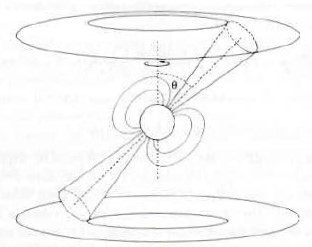
\includegraphics{pulsar.jpg}
    \caption{A pulsar \autocite{maoz}.}
    \label{fig:pulsar1}
\end{figure}

While some pulsars, like the Crab Pulsar \autocite{maoz}, emit electromagnetic waves in the visible spectrum and can therefore be detected by an optical telescope, the majority of pulsar emission is invisible to the human eye and requires a radio telescope to be detected.

\subsubsection{What is a Pulsar Profile?}
\subsubsection{What is multi-path scattering?}
\subsubsection{What is a Pulsar Dispersion Measure?}
\subsubsection{What is a Radio Telescope and how do they work?}
\subsubsection{What is the Murchison Widefield Array?}
\subsubsection{Why are we conducting sky surveys?}
\subsubsection{How is a sky survey conducted with the Murchison Widefield Array?}
\subsubsection{What is tied-array beamforming?}
\subsubsection{How many Pulsar candidates are found in a Murchison Widefield Array sky survey?}
\subsubsection{How long do sky surveys take?}
\subsubsection{How much data is created from a sky survey?}
\subsubsection{What is Radio Frequency Interference?}
\subsubsection{What is a Signal-to-Noise Ratio?}
\subsubsection{What is PRESTO and a .PFD file?}
\subsubsection{What is Machine Learning?}
\subsubsection{How does Machine Learning work?}
\subsubsection{Why do we need to use Machine Learning in finding new Pulsars?}
\subsubsection{Why is this particular Machine Learning Classifier used?}


\pagebreak
% Methods Section
\section{Methods}
\subsection{Developing the MWA Machine Learning Training\\ Datasets}
\subsubsection{Pulsar Candidate Training Datasets}
\subsubsection{RFI Training Dataset}
\subsubsection{Noise Training Dataset}
\subsection{Evaluating the LOFAR Machine Learning Algorithm for use with the MWA}

\pagebreak
% Results Section
\section{Results}
\subsection{Pulsar Candidate Training Dataset}
\subsection{Radio Frequency Interference Training Dataset}
\subsection{Noise Training Dataset}
\subsection{Output from LOFAR Algorithm with MWA Data}
\subsection{Adaptations to the Machine Learning Algorithm}

\pagebreak
% Results Discussion Section
\section{Discussion}
\subsection{How effective are the training datasets?}
\subsection{Why didn't the LOFAR Machine Learning Algorithm work with the MWA?}
\subsection{What changes to the algorithm were necessary for it to successfully classify Pulsars from the MWA?}

\pagebreak
% FINAL CONCLUSTIONS SECTION
\section{Conclusions}

% RECOMMENDATIONS SECTION
\section{Recommendations}

\pagebreak
% REFERENCES SECTION
\section{References}
\printbibliography[heading=none]

\pagebreak
% APPENDICES SECTION
\section{Appendices}
\subsection{Pulsar Feature Lab}
\subsection{Pulsar Classifier}

% End the document
\end{document}